@% Chapter 5

\chapter{Aplicação} % Main chapter title
\label{chap:Chapter5} % For referencing the chapter elsewhere, use \ref{chap:Chapter5} 

%----------------------------------------------------------------------------------------
\section{Sistema Desenvolvido}
O objetivo principal da parte prática da dissertação é não só recolher sinais e criar a sua função de ambiguidade, mas principalmente detetar um objeto estático e em movimento.
Para realizar estas tarefas foi utilizado um transmissor e recetor LimeSDR USB. As suas principais caraterísticas estão apresentadas na seguinte tabela e a sua documentação em \url{https://wiki.myriadrf.org/LimeSDR-USB}.\par

\begin{table}[h]
\centering
\begin{tabular}{@{}ccccc@{}}
\toprule
Caraterística       			 & Descrição                      \\ \midrule
\textit{RF Transreceiver}        & LMS7002M                       \\
\textit{Oscillator}    			 & Rakon RPT7050A @30.72$MHz$    \\
Banda de frequência              & 100$kHz$ - 3.8$GHz$            \\ 
Largura de banda máxima          & 61.44$MHz$                     \\ \bottomrule
\label{tab:limesdr}
\end{tabular}
\caption[Caraterísticas do LimeSDR USB]{Caraterísticas do LimeSDR USB}
\end{table}

Por forma a reduzir o ruído a alimentação é feita através dum \textit{power bank} de 20000$mAh$. Isto é conseguido com um cabo em "Y" que vem com o LimeSDR, que separa a entrada de dados da alimentação do equipamento.\par 
As duas antenas utilizada tanto para o canal de receção do sinal direto como do sinal refletido são antenas \textit{One for all} \textit{Yagi} de exterior para televisão, com $24dB$.\par 
Para a ligação entre o \textit{LimeSDR} e as antenas foram utilizados cabos coaxiais RG-58 com $1m$ de comprimento onde foram cravadas fichas SMA, como representado na figura \ref{fig:limec}.\par 
O repositório que contém as drivers que permitem trabalhar com o LimeSDR a partir do MATLAB foram desenvolvidos inicialmente e disponibilizado no link \url{https://github.com/jocover/Simulink-MATLAB-LimeSDR} em Agosto de 2017 pelo autor Jocover, posteriormente adaptado e atualizado em Dezembro de 2019 pelo autor Damir Rakhimov para a versão do LimeSuite 19.04 e pode ser acedido no \textit{github} do mesmo, \url{https://github.com/RakhDamir/LimeSDR-Matlab}. Todos os passos de instalação e configuração do sistema encontram-se disponibilizados no seu \textit{github}.

\begin{figure}[h]
\centering
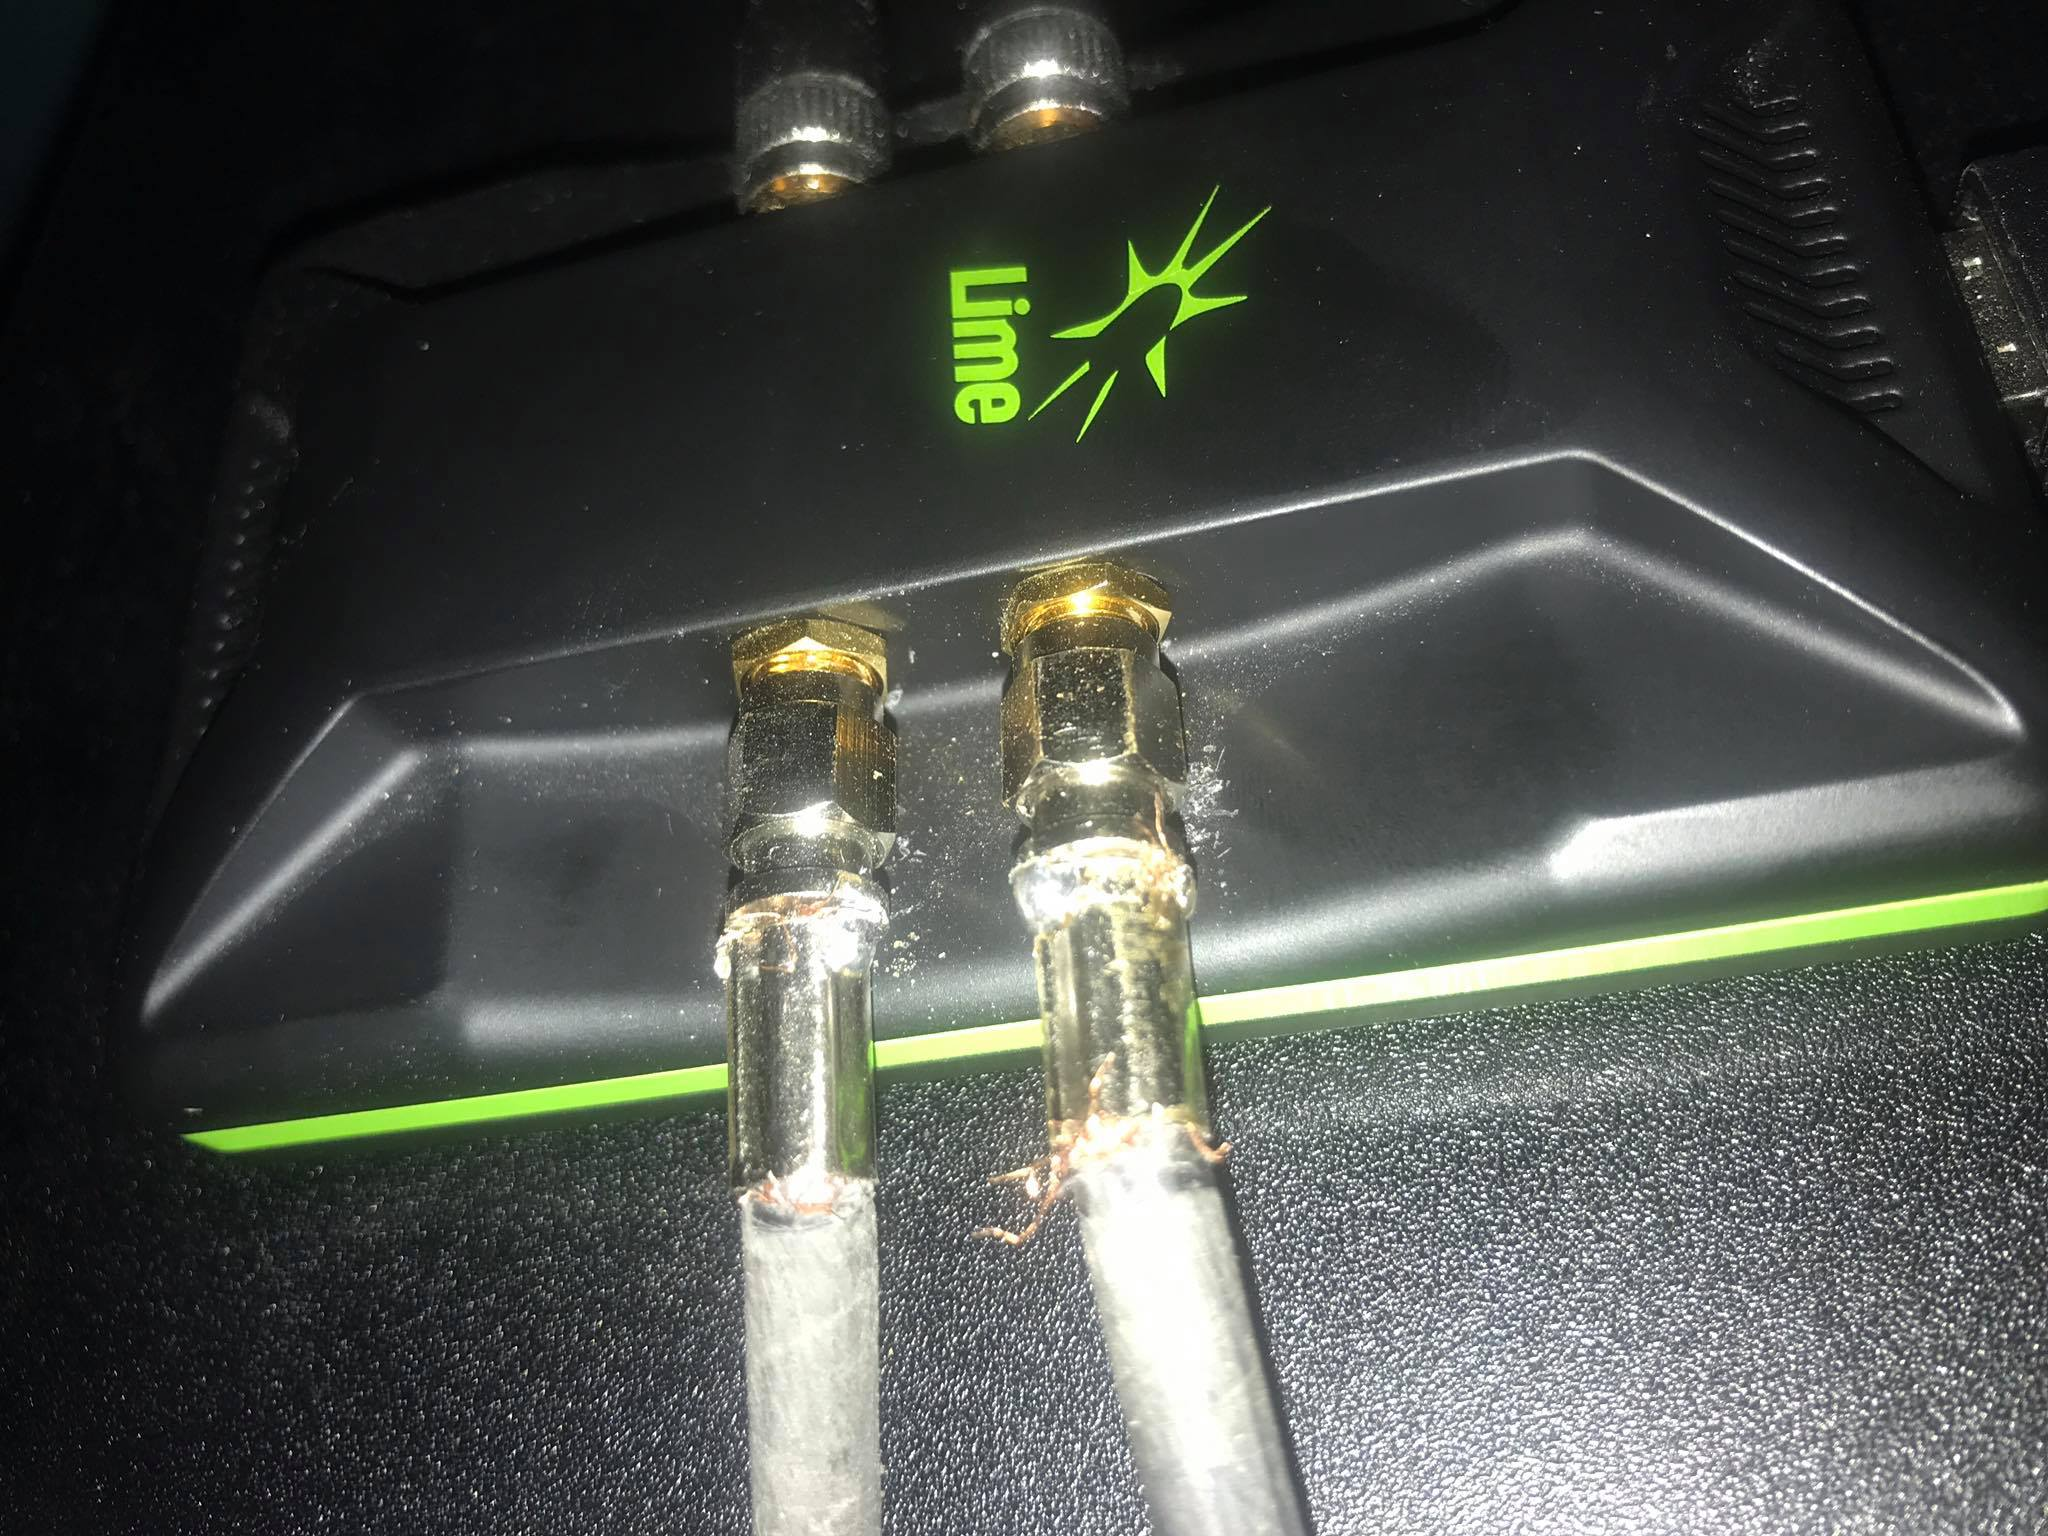
\includegraphics[scale=0.15]{chapters/ch5/assets/limec}
\caption[Entrada LimeSDR]{Entrada LimeSDR}
\label{fig:limec}
\end{figure}

Para o estudo da deteção de alvos utilizando sistemas de deteção passivos, foi utilizado sinais \gls{DVB-T} dos transmissores de Palmela (38°33'23.02"N	8°54'27.56"W) e Cruz de Pau (38°37'3.78"N	9°7'2.31"W), ambos a transmitir nas frequências $598-606 MHz$, e a posição do estudo foi em Brejos de Azeitão (38°32'11.10"N	9°1'21.43"W). Para uma melhor compreensão do panorama geográfico, a imagem \ref{fig:mapaemi} representa os transmissores a amarelo,  os utilizados a amarelo com um risco preto por baixo e a posição da experiência com um círculo azul.


\begin{figure}[h]
\centering
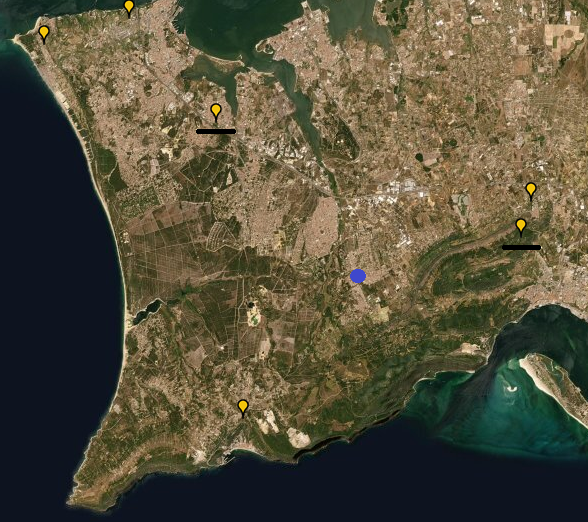
\includegraphics[scale=0.8]{chapters/ch5/assets/mapaemi}
\caption[Mapa de emissores e local da experiência]{Mapa de emissores e local da experiência}
\label{fig:mapaemi}
\end{figure}

\section{Resultados}
